\documentclass[landscape]{article}
% For rotating figures, tables, etc.
%  including their captions
\usepackage[margin=1in]{geometry}

\usepackage{tikz}
\usepackage{tcolorbox}
\usepackage{setspace}
\usepackage{ragged2e}
\usepackage{overpic}

% --- Tikz stuff
\usetikzlibrary{shapes.geometric, hobby, decorations.pathreplacing, calc}
\usetikzlibrary{arrows, arrows.meta}
\usetikzlibrary{shapes.multipart}

\definecolor{sapphire}{HTML}{0F52BA}
\definecolor{emerald}{HTML}{27AE60} % 229954} % 50C878}

\begin{document}
\begin{minipage}{.6\textwidth}
    \begin{tikzpicture}[scale=1]

        % upper grid
        \node(upper) at (-1, 1){
            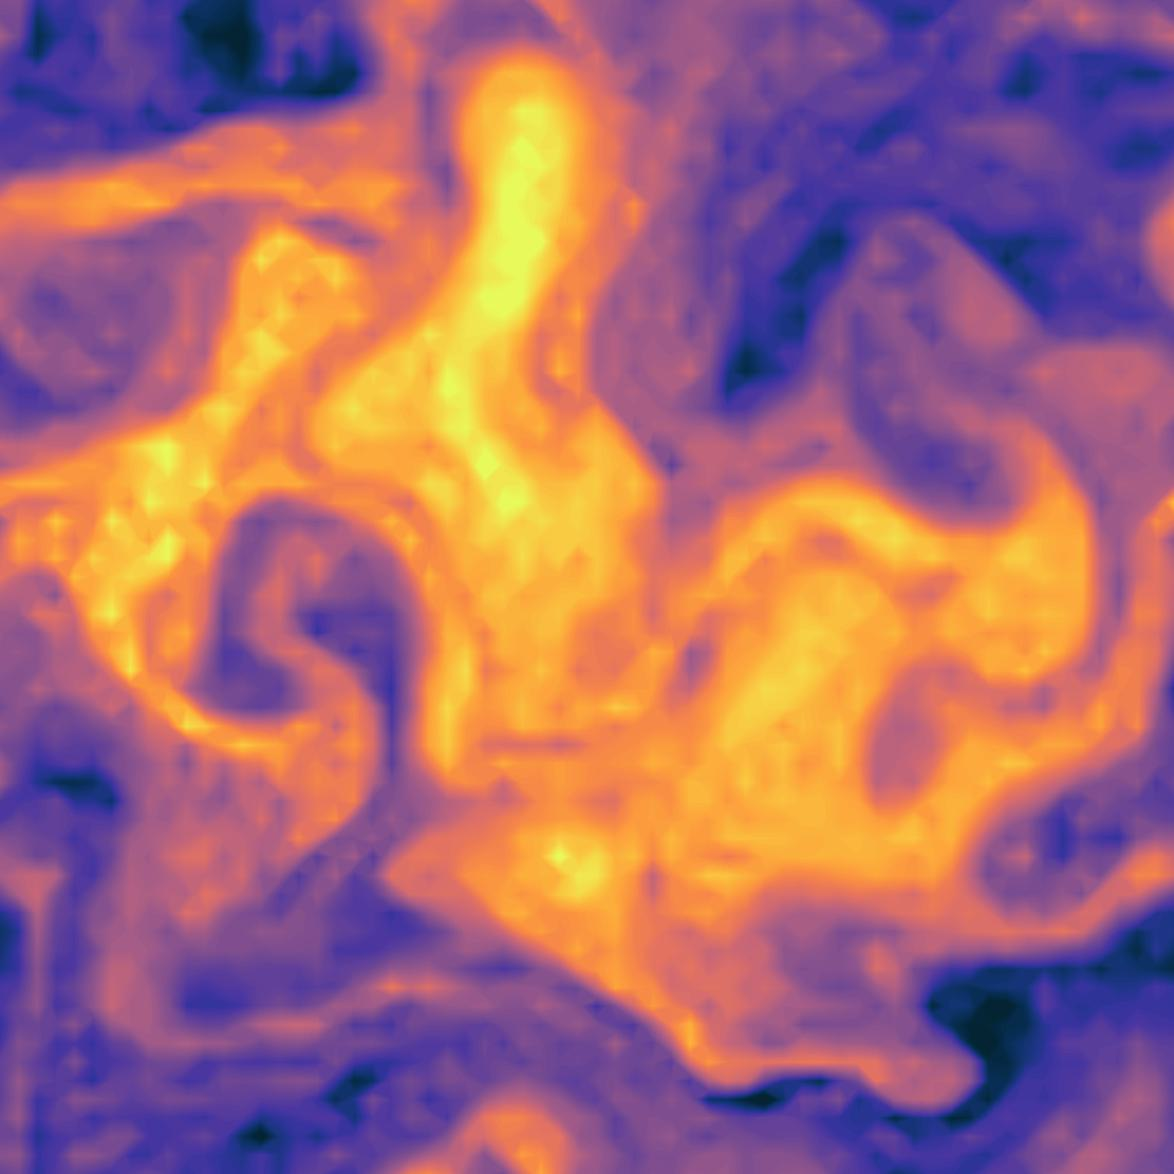
\includegraphics[width=.73\textwidth]{../theta-z1.jpg}
        };
        \draw[line width=4pt, xshift=-1cm, yshift=1cm, draw=black] (-5, -5) grid[step=2.5] +(10,10);

        % overlap
        \draw[white, line width=4pt] (-4, 0.5) rectangle (-0.5, 4);


        % lower grid
        \node(lower) at (1, -1){
            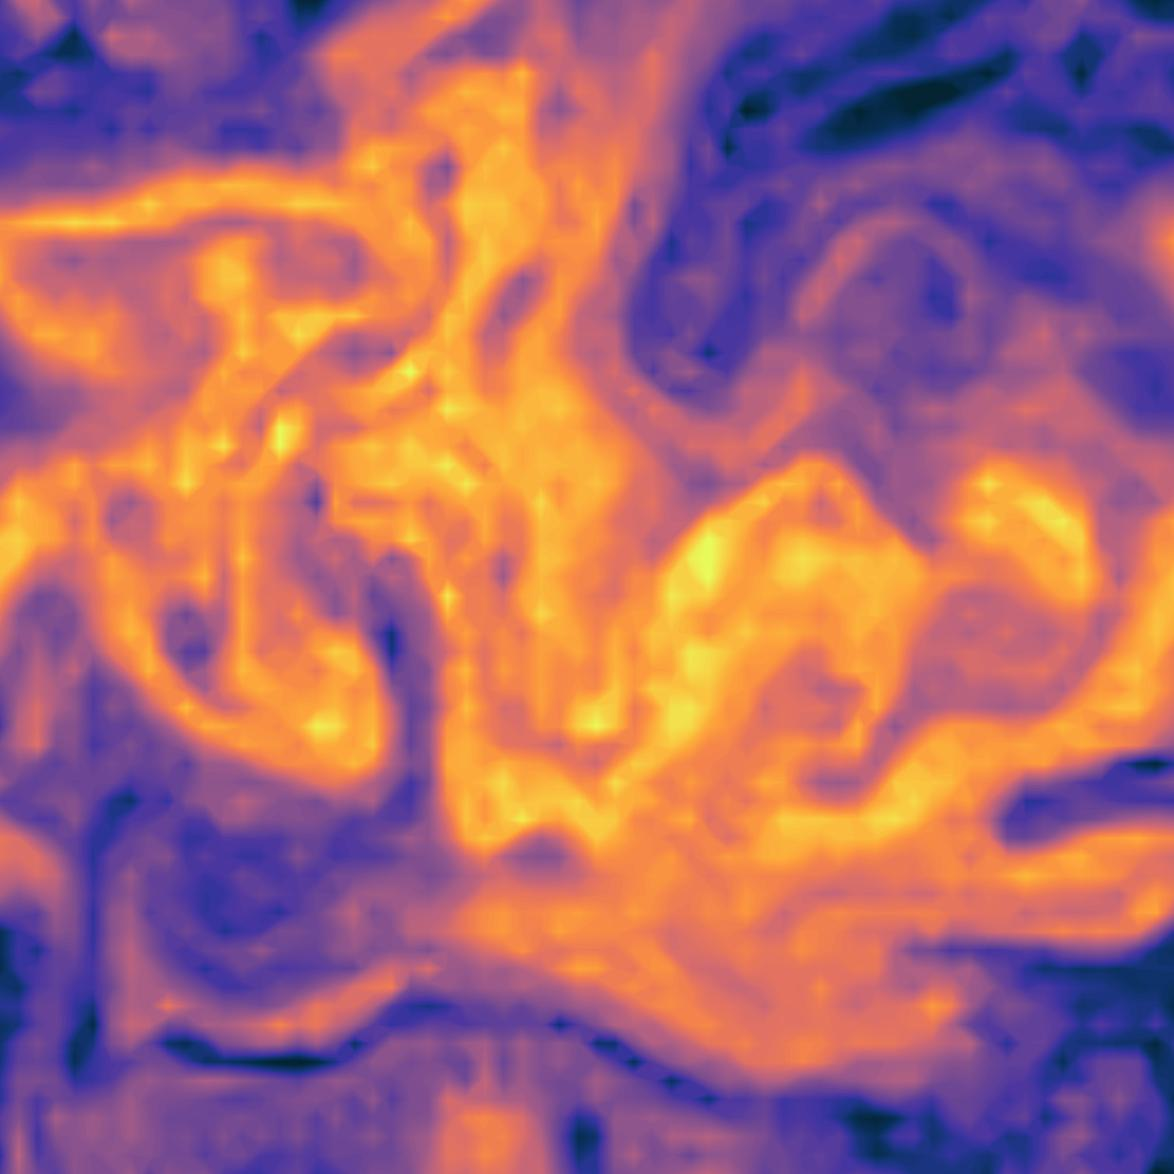
\includegraphics[width=.72\textwidth]{../theta-z0.jpg}
        };

        \draw[line width=4pt, xshift=-1.5cm, yshift=-1cm, draw=black] (-2.5, -5) grid[step=2.5] +(10,10);

        % overlap
        \draw[white, line width=4pt] (-2, -1.5) rectangle (1.5, 2);

        % left z dim
        \draw [line width=4pt]
            ($ (upper.south west) + (0.1, 0.16) $)
            --
            ($ (lower.south west) + (0.1, 0.05) $);

        \draw [line width=4pt]
            ($ (upper.south west) + (0.1, 2.66) $)
            --
            ($ (lower.south west) + (0.1, 2.55) $);

        \draw [line width=4pt]
            ($ (upper.south west) + (0.1, 5.16) $)
            --
            ($ (lower.south west) + (0.1, 5.05) $);

        \draw [line width=4pt]
            ($ (upper.south west) + (0.1, 7.66) $)
            --
            ($ (lower.south west) + (0.1, 7.55) $);

        \draw [line width=4pt]
            ($ (upper.south west) + (0.1, 10.16) $)
            --
            ($ (lower.south west) + (0.1, 10.05) $);

        % upper  z dim
        \draw [line width=4pt]
            ($ (upper.south west) + (2.6, 10.16) $)
            --
            ($ (lower.south west) + (2.6, 10.05) $);

        \draw [line width=4pt]
            ($ (upper.south west) + (5.1, 10.16) $)
            --
            ($ (lower.south west) + (5.1, 10.05) $);

        \draw [line width=4pt]
            ($ (upper.south west) + (7.6, 10.16) $)
            --
            ($ (lower.south west) + (7.6, 10.05) $);

        \draw [line width=4pt]
            ($ (upper.south west) + (10.1, 10.16) $)
            --
            ($ (lower.south west) + (10.1, 10.05) $);

        % --- Labels
        \draw [line width=4pt,
            {Stealth}-{Stealth}]
            ($ (lower.south east) - (2.5, 0.5) $)
            --
            ($ (lower.south east) - (.25, 0.5) $)
            node [midway, yshift=-3em] {\Huge $N_x^{loc} = 16$};

        \draw [line width=4pt,
            {Stealth}-{Stealth}]
            ($ (lower.south east) + (0.5, .25) $)
            --
            ($ (lower.south east) + (0.5, 2.5) $)
            node [midway, xshift=8em] {\Huge $N_y^{loc} = 16$};

        \draw [line width=5pt,
            {Stealth}-{Stealth}]
            ($ (upper.north west) + (0.45, 0.5) $)
            --
            ($ (upper.north east) - (0.45, -0.5) $)
            node [midway, yshift=2em] {\Huge $N_x = 64$};

        \draw [line width=5pt,
            {Stealth}-{Stealth}]
            ($ (upper.south west) + (-0.5, 0.45) $)
            --
            ($ (upper.north west) - (0.5, 0.45) $)
            node [midway, xshift=-2em, rotate=90] {\Huge $N_y = 64$};
        \draw [line width=5pt,
            {Stealth}-{Stealth}]
            ($ (upper.south west) - (0.5, 0.5) $)
            --
            ($ (lower.south west) - (0.5, 0.5) $)
            node [midway, xshift=-2em, yshift=-2em, rotate=-45] {\Huge $N_z = 2$};
    \end{tikzpicture}
\end{minipage}

\end{document}
